\subsection{MF POS short sequences \label{sec:pos_short_sequences}}

Another possible stylistic aspect that can be detected is to consider the sentence constructions.

\subsubsection{Method}

This can be solved by creating a short POS sequences text representation.
Used in conjonction with the MF method, this can produce feature vetors which can be used to compare documents.

These short sequences are created using the same principal used for the $n$-grams.
From a list of POS, each POS is considered as a letters when applying the $n$-grams algorithm.
This type of $n$-grams is also known as w-shingling.

For example, the sentence : \textit{"The cat eat a fish"} has the following POS tag \textit{"Article Noun Verb Article Noun"} which correspond to the following short POS sequences of size 3 : \textit{"Article Noun Verb"} / \textit{"Noun Verb Article"} / \textit{"Verb Article Noun"}.

In practice the POS is more detailed, for example instead of just considering \textit{eat} as a verb, a more detailed POS can be the verb and its tense \textit{Verb-SimplePresent}, the same goes for the other type of POS.

For the sake of simplicity, in this study, a POS short sequence of size $n$ is written $n$-POS.

The MF method can be applied to the $n$-POS text representation to turn each document into a feature vector.
Than they can be compared using distance metrics to find distance between documents.

\subsubsection{Evaluation}

For this experiment, $n$-POS are used to detect the style of the author.

$1$-POS are discarded from the experiment (equivalent of the POS frequency) since previous studies showed that $1$-POS tends to produce worse results then with larger $n$~\cite{kocher_linking}.

To lower the computational cost, this evaluation is split in two parts, the first aim to select the most convincing size of $n$-POS and the best fitting $n$-MF.
The second is to compare the different distance metrics.
Keep in mind, as for the previous experiment in two parts, this experimentation methodology ignore the strength and weakness of distance measure with regard to the dimensionality of the vectors.

\textbf{First part}

In the first part, only $2$-POS, $3$-POS, $4$-POS and the combination of the $2$-POS and $3$-POS denoted: $(2, 3)$-POS are used.
The distance metric used for this part is the smoothed Z-Score normalized Cosine distance.
For this representation no clear $n$-MF vector size is advised, the size used is between 200 and 2000 with a step of 100.

Figure~\ref{fig:n_pos} show the average precision on the rank list produced by using $n$-POS over the $n$-MF.

The two following information can be intuitively observed on this plot:
\begin{itemize}
  \item
  The $(2, 3)$-POS have similar resutls to the $3$-POS method.
  Due to its larger text representation, the $(2, 3)$-POS can already be discarded.
  \item
  A larger / more complex $n$-POS require a larger $n$-MF to achieve its maximal effectiveness.
  In the St-Jean corpus, a total of 26 different POS are used to describe every words in the corpus.
  Which correspond to $26^2 = 676$ possible unique $2$-POS, to $26^3 = 17,576$ $3$-POS and $26^4 = 456,976$ $4$-POS, thus $2$-POS converges and not $3$/$4$-POS.
  \item
  Like other methods, if the $n$-MF is too large, an overfitting to less important items is possible, thus reducing the average precision.
  In Figure~\ref{fig:n_pos} the $2$-POS clearly have a drop in average precision after $\sim 250$-MF.
\end{itemize}

Using the smoothed Z-Score Cosine distance, the most appropriate configuration for the $n$-POS text representation on St-Jean is $2$-POS with $250$-MF and $3$-POS with $1000$-MF .

\begin{figure}
  \centering
  \caption{Average precision over the $n$-MF for the rank list generated using the Z-Score normalized Cosine distance on St-Jean's $n$-POS text representation.}
  \label{fig:n_pos}
  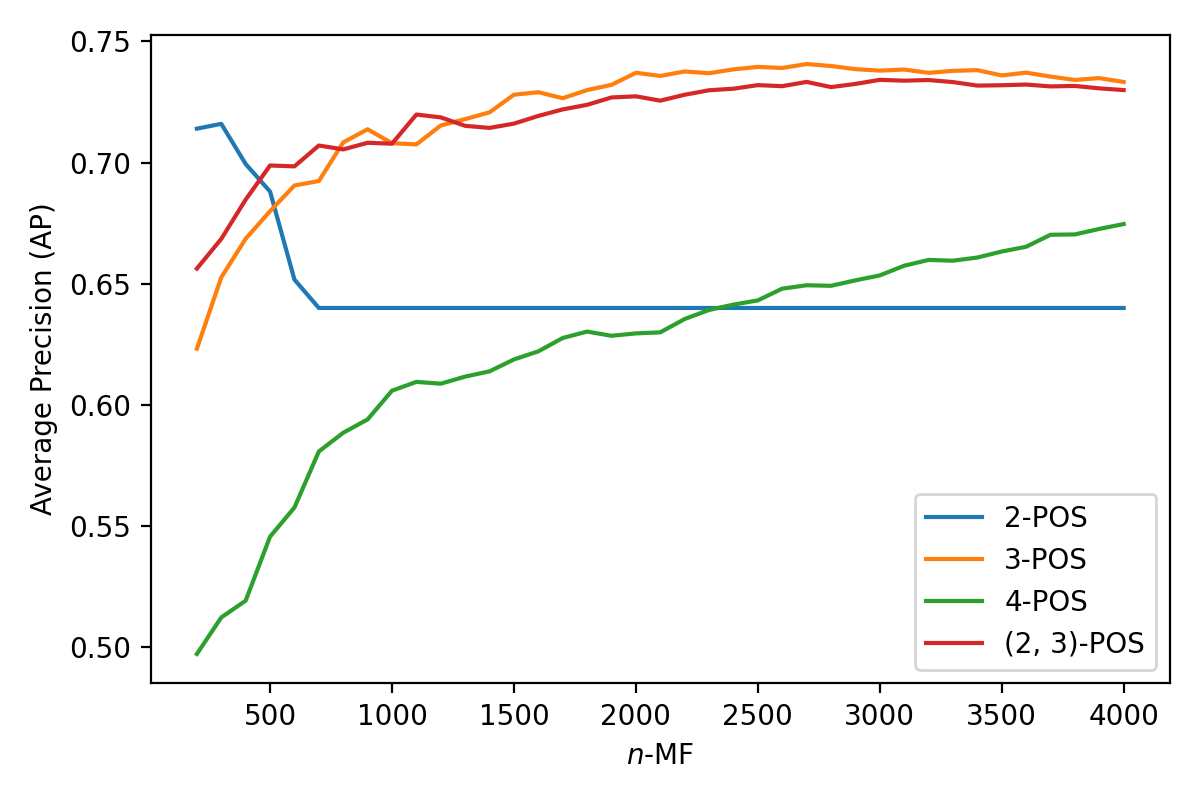
\includegraphics[width=\linewidth]{img/n_pos.png}
\end{figure}

\textbf{Second part}

In this second part, the goal is to find the most appropriate distance metric for the $n$-POS text representation, with the configuration retained in the first part.
After running with these parameters on every proposed distance metrics, Table~\ref{tab:n_pos} shows a resume of the experiment.

When considering $n$-POS as text representation on the St-Jean corpus, over all the best distance metrics are Manhattan, Matusita, Cosine distance.
The Clark distance, give overall the worse results, even though in other text representation, this metric was giving the best results.

Optimizing the parameters with this text representation can increase the average precision by up to $36$\% in average.

Two configurations are retained using the $n$-POS text representation.
The first is the $2$-POS with $250$-MF and the smoothed Z-Score Cosine Distance.
And the second is $3$-POS $1000$-MF using the smoothed Z-Scored Manhattan distance.

\begin{table}
  \centering
  \caption{Average precision for every distance metrics with the $n$-POS representation on St-Jean}
  \label{tab:n_pos}
  \begin{tabular}{l c c c}
    \toprule
                    & \multicolumn{2}{c}{$n$-POS/$n$-MF} \\
    Distance metric & $2$-POS/$250$-MF & $3$-POS/$1000$-MF \\
    \midrule
    Manhattan & 0.70 & \textbf{0.75} \\
    Tanimoto & 0.67 & 0.72 \\
    Euclidean & 0.69 & 0.72 \\
    Matusita & 0.70 & 0.73 \\
    Clark & 0.50 & 0.60 \\
    Cosine & \textbf{0.73} & 0.71 \\
    KLD & 0.68 & 0.70 \\
    JD & 0.69 & 0.73 \\
    \bottomrule
  \end{tabular}
\end{table}
